\usetheme[numbering=fraction]{metropolis}

\metroset{block=fill}

\usepackage[dvipsnames]{xcolor}

\usepackage{booktabs}

\usepackage{fancyvrb}
\fvset{listparameters=\setlength{\topsep}{0pt}\setlength{\partopsep}{0pt}}

\usepackage{csquotes}
\setquotestyle{british}

\usepackage{graphicx}
\graphicspath{ {../../images/} }

\usepackage{pgfplots}
\usetikzlibrary{positioning,calc,external}
%\tikzexternalize[prefix=figures/] 

\usepackage{crysymb}

\renewcommand*{\arraystretch}{1.2}

\usepackage{soul}
\usepackage[en-GB]{datetime2}
\DTMlangsetup[en-GB]{ord=omit}

\usetikzlibrary{positioning,calc}
\graphicspath{ {../../images/} }

\title{ICS0026 Cryptography}
\subtitle{TLS, CT and CAA}
\date{\DTMdate{2024-03-26}}
\author{Taaniel Kraavi}
\institute%
{%
  \textit{IT College}\\
  \textit{Tallinn University of Technology}
}

\begin{document}
\begin{frame}
  \titlepage
\end{frame}

\begin{frame}{Securing traffic on the web}
  How do we create a secure communication channel over a network?

  \vspace*{1em}

  \pause
  What do we protect against?
  \begin{itemize}[<+(1)->]
    \item Eavesdropping
    \begin{itemize}
      \item $\implies$ Confidentiality
    \end{itemize}
    \item Tampering
    \begin{itemize}
      \item $\implies$ Integrity \& authenticity
      \item Integrity must be authenticated (accidental vs. malicious modifications)
    \end{itemize}
    \item Impersonation/forgery
    \begin{itemize}
      \item $\implies$ Authenticity
    \end{itemize}
  \end{itemize}

  \vspace*{1em}

  \pause
  We need a \emph{protocol} satisfying these requirements.
\end{frame}

\begin{frame}{SSL \& TLS}
  Secure Sockets Layer (SSL) by Netscape
  \begin{itemize}[<+(1)->]
    \item SSL 1.0 never released (security flaws)
    \item SSL 2.0 (1995) deprecated in 2011 (\href{https://datatracker.ietf.org/doc/html/rfc6176}{RFC 6176})
    \item SSL 3.0 (1996) deprecated in 2015 (\href{https://datatracker.ietf.org/doc/html/rfc7568}{RFC 7568}) 
  \end{itemize}

  \vspace*{1em}

  \pause
  Transport Layer Security (TLS)
  \begin{itemize}[<+(1)->]
    \item Born out of SSL 3.0 to replace it
    \item TLS 1.0 (1999) \& TLS 1.1 (2006), deprecated in 2021 (\href{https://datatracker.ietf.org/doc/html/rfc8996}{RFC 8996})
    \item TLS 1.2 (2008, \href{https://datatracker.ietf.org/doc/html/rfc5246}{RFC 5246}) not yet deprecated, but should
    \item TLS 1.3 (2018, \href{https://datatracker.ietf.org/doc/html/rfc8446}{RFC 8446}) obsoletes TLS 1.2
  \end{itemize}
\end{frame}

\begin{frame}{Transport Layer Security (TLS)}
  TLS is a cryptographic \emph{protocol}.
  \begin{itemize}[<+(1)->]
    \item Used for securing HTTPS, email, VoIP, instant messaging, \dots
    \item Assumes a reliable transport protocol (e.g. TCP)
    \item Datagram TLS (DTLS)
    \begin{itemize}
      \item `TLS for stream-communications' e.g. UDP
      \item \href{https://datatracker.ietf.org/doc/html/rfc9147}{RFC 9147} for DTLS 1.3 (2022)
      \item Security guarantees of TLS except for order protection / non-replayability
    \end{itemize}
  \end{itemize}

  \vspace*{1em}

  \pause
  Connections are negotiated with the \emph{TLS handshake}.
  \begin{itemize}[<+(1)->]
    \item Client and server agree on parameters
    \item The subsequent connection is \emph{stateful}
  \end{itemize}
\end{frame}

\begin{frame}{TLS handshake overview}
  The client and server agree on the following:
  \begin{itemize}[<+(1)->]
    \item TLS version to use (1.2 or 1.3)
    \begin{itemize}
      \item Downgrade attacks are a reason why 1.2 should be deprecated
    \end{itemize}
    \item Cipher suite to use
    \begin{itemize}
      \item Set of algorithms for establishing the secure connection
      \item Client and server agree on what they both support
    \end{itemize}
    \item Authenticate the server's identity
    \begin{itemize}
      \item Server's public key \& CA's digital signature
    \end{itemize}
    \item Create session keys
    \begin{itemize}
      \item These protect the actual communication session
    \end{itemize}
  \end{itemize}
\end{frame}

\begin{frame}{TLS 1.3 handshake with DH}
  \begin{figure}
    \center
    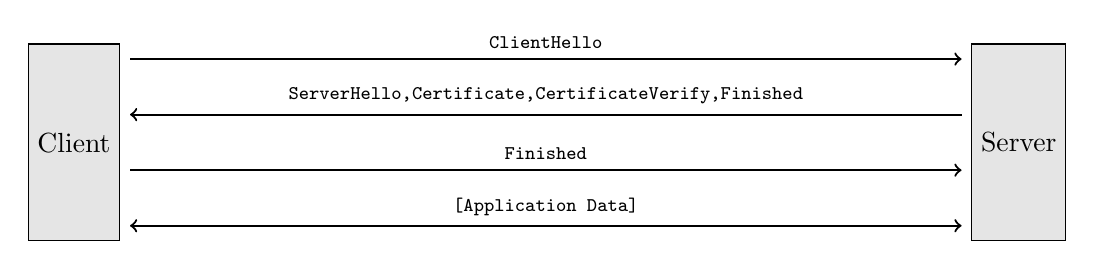
\begin{tikzpicture}
      \node[draw,minimum height=2.5cm,fill=gray!20] (client) at (0,0)   {Client};
      \node[draw,minimum height=2.5cm,fill=gray!20] (server) at (12, 0) {Server};

      \node (A) at (client.east) [yshift=30px] {};
      \node (B) at (server.west) [yshift=30px] {};
      \node (C) at (client.east) [yshift=10px] {};
      \node (D) at (server.west) [yshift=10px] {};
      \node (E) at (client.east) [yshift=-10px] {};
      \node (F) at (server.west) [yshift=-10px] {};
      \node (G) at (client.east) [yshift=-30px] {};
      \node (H) at (server.west) [yshift=-30px] {};

      \draw[->,thick]  (A) -- (B) node[midway,above] {\scriptsize\texttt{ClientHello}};
      \draw[<-,thick]  (C) -- (D) node[midway,above] {\scriptsize\texttt{ServerHello,Certificate,CertificateVerify,Finished}};
      \draw[->,thick]  (E) -- (F) node[midway,above] {\scriptsize\texttt{Finished}};
      \draw[<->,thick] (G) -- (H) node[midway,above] {\scriptsize\texttt{[Application Data]}};
    \end{tikzpicture}
  \end{figure}

  \vspace*{1em}

  \begin{itemize}[<+(1)->]
    \item {\small\texttt{ClientHello}}: nonce, client's DH share, and supported parameters
    \item {\small\texttt{ServerHello}}: negotiated connection parameters, server's DH share
    \item {\small\texttt{CertificateVerify}}: signature over the entire handshake
    \item {\small\texttt{Finished}}: MAC over the entire handshake
    \item Other approaches exist (e.g. based on PSK instead of DH)
  \end{itemize}
\end{frame}

\begin{frame}{Major fixes by TLS 1.3}
  \begin{itemize}
    \item Legacy symmetric encryption algorithms pruned
    \begin{itemize}
      \item Only AEAD schemes remain
    \end{itemize}
    \item De-facto inclusion of ECC, e.g. EdDSA
    \item Various crypto improvements
    \begin{itemize}
      \item RSA-PSS instead of PKCS\#1 v1.5
      \item Removed DSA, EC point compression \& custom DHE groups
    \end{itemize}
    \item Perfect forward secrecy by default (static cipher suites removed)
    \begin{itemize}
      \item For (EC)DHE and PSK with (EC)DHE (but not PSK-only)
    \end{itemize}
    \item Encryption of handshake messages after the Server Hello
    \item Simplified handshake in general
    \item Dropped renegotiation support
    \item \dots
  \end{itemize}
\end{frame}

\begin{frame}{Perfect forward secrecy (PFS)}
  A hybrid problem:
  \begin{itemize}[<+(1)->]
    \item Servers have long-term keys, e.g. for signing
    \item Client encrypts shared key and sends to the server (static RSA)
    \item If the server key is compromised, all previous shared keys can be recovered
  \end{itemize}

  \vspace*{1em}

  \pause
  PFS prevent past comms from being decrypted if long-term keys leak.
  \begin{itemize}[<+(1)->]
    \item Generate a new key for each communication session (ephemeral key)
    \item Discard the keys after the session
    \item TLS 1.3 has PFS by default (except for PSK-only)
  \end{itemize}
\end{frame}

\begin{frame}{TLS 1.3 cipher suites}
  TLS v1.3 supports 5 cipher suites:
  \pause
  \begin{itemize}
    \item {\small\texttt{TLS\_AES\_256\_GCM\_SHA384}}
    \item {\small\texttt{TLS\_CHACHA20\_POLY1305\_SHA256}}
    \item {\small\texttt{TLS\_AES\_128\_GCM\_SHA256}}
    \pause
    \item {\small\texttt{TLS\_AES\_128\_CCM\_8\_SHA256}} (not enabled by default)
    \item {\small\texttt{TLS\_AES\_128\_CCM\_SHA256}} (not enabled by default)
  \end{itemize}

  \pause
  TLS 1.2 specified 37\dots
  \begin{itemize}[<+(1)->]
    \item Confusing nomenclature
    \item E.g. {\small\texttt{TLS\_ECDHE\_RSA\_WITH\_AES\_128\_GCM\_SHA256}}
  \end{itemize}
\end{frame}

\begin{frame}{Some resources}
  Checking TLS 1.3 support:
  \begin{itemize}
    \item {\small\url{https://caniuse.com/tls1-3}} for browser support
    \item \href{https://support.globalsign.com/ssl/general-ssl/tls-protocol-compatibility}{GlobalSign's reference}
    \item \href{https://learn.microsoft.com/en-us/windows/win32/secauthn/protocols-in-tls-ssl--schannel-ssp-}{Windows support table}
  \end{itemize}

  \pause
  Testing a website's configuration:
  \begin{itemize}
    \item {\small\url{https://www.ssllabs.com/ssltest/}}
    \item {\small\url{https://www.hardenize.com}}
  \end{itemize}

  \pause
  Some cipher suite recommendations (for TLS 1.2 support)
  \begin{itemize}
    \item \href{https://developers.cloudflare.com/ssl/reference/cipher-suites/recommendations/}{Cloudflare recommendations}
    \item \href{https://www.iana.org/assignments/tls-parameters/tls-parameters.xhtml?ref=hackernoon.com\#tls-parameters-4}{IANA recommendations}
  \end{itemize}
\end{frame}

\begin{frame}{Root programs}
  \pause
  Which CA's to trust by default?
  \begin{itemize}[<+(1)->]
    \item \href{https://aka.ms/RootCert}{Microsoft Trusted Root Program}
    \item \href{https://www.apple.com/certificateauthority/ca_program.html}{Apple Root Certificate Program}
    \item \href{https://wiki.mozilla.org/CA}{Mozilla's CA Certificate Program}
    \item \href{https://g.co/chrome/root-policy}{Chrome Root Program}
    \item \dots
  \end{itemize}
\end{frame}

\begin{frame}{Some CA's}
  Popular CAs for TLS certificates:
  \begin{itemize}[<+(1)->]
    \item IdenTrust
    \item Let's Encrypt\textsuperscript{*}
    \item GlobalSign
    \item Sectigo
    \item DigiCert
    \item GoDaddy
  \end{itemize}
  
  \vfill

  \pause
  Market share yearly trends for SSL certificate authorities:

  {\scriptsize\url{https://w3techs.com/technologies/history_overview/ssl_certificate/ms/y}}
\end{frame}

\begin{frame}{Web certificate types}
  Domain validated (DV)
  \begin{itemize}[<+(1)->]
    \item Proof of control over WhoIS records
    \item Typical confirmation: DNS record, email contact (e.g. whois, webmaster@), \dots
    \item Free these days (e.g. Let's Encrypt)
  \end{itemize}

  \pause
  Organisation validated (OV)
  \begin{itemize}[<+(1)->]
    \item Verification of org's name and registration status
  \end{itemize}

  \pause
  Extended validated (EV)
  \begin{itemize}[<+(1)->]
    \item Selected CAs, verification of legal identities, physical presence, \dots
    \item {\scriptsize\url{https://cabforum.org/working-groups/server/extended-validation/documents/}}
  \end{itemize}

  \pause
  Modern browsers no longer make visual distinctions between the types.
\end{frame}

\begin{frame}{Let's Encrypt}
  \pause
  Let's Encrypt is a free, automated, and open certificate authority brought to you by the nonprofit Internet Security Research Group (ISRG). ({\scriptsize\url{https://letsencrypt.org}})
  \begin{itemize}[<+(1)->]
    \item Provide DV TLS certificates to any compatible client
    \begin{itemize}
      \item Verifies domain ownership via unique tokens
      \item Tokens validated over web/DNS requests
    \end{itemize}
    \item Automated using ACME (Automatic Certificate Management Environment)
    \item \href{https://certbot.eff.org}{Certbot}
    \begin{itemize}
      \item Convenient ACME client
      \item Automatic TLS configuration on Nginx/Apache
      \item Other ACME clients exist
    \end{itemize}
  \end{itemize}

  \pause
  No excuse to have a non-HTTPS website.
\end{frame}

\begin{frame}{Certificate transparency (CT)}
  What if a CA starts falsely issuing certificates?
  \begin{itemize}[<+(1)->]
    \item Certificate transparency (CT)
    \item Public log of certificates issued by trusted CAs
    \begin{itemize}
      \item Logs are append-only
      \item Operated by browser vendors and CAs themselves
    \end{itemize}
    \item Signed certificate timestamp (SCT)
    \begin{itemize}
      \item Signed by another log operator
      \item Inclusion in a log within a maximal delay
    \end{itemize}
    \item Identification of mistakenly/maliciously issued certificates
    \begin{itemize}
      \item {\small{\url{https://certificate.transparency.dev/monitors/}}}
    \end{itemize}
  \end{itemize}
\end{frame}

\begin{frame}{Certificate pinning}
  For the `highest' trust level, certificates and keys can be pinned.
  \begin{itemize}[<+(1)->]
    \item Client device contains a list of approved certificates
    \begin{itemize}
      \item e.g. Estonian i-voting client
    \end{itemize}
    \item `Precursor' to certificate transparency
    \begin{itemize}
      \item HTTP Public Key Pinning
      \item HTTP header with public key hashes
      \item Obsoleted in favour of CT
    \end{itemize}
    \item Generally not practical:
    \begin{itemize}
      \item Lack of flexibility and scalability
      \item Complex and risky (what to do in case of issues?)
    \end{itemize}
    \item OCSP stapling and CT are generally sufficient
  \end{itemize}
\end{frame}

\begin{frame}{Certification Authority Authorization (CAA)}
  CT allows us to be reactive.
  Can we be proactive?
  \begin{itemize}
    \item Certification Authority Authorization (CAA)
    \item \href{https://datatracker.ietf.org/doc/html/rfc8659}{RFC 8659}
    \item Specify in DNS which CAs can issue certificates for the domain
    \begin{itemize}
      \item Compliant CAs must not issue certificates when unauthorised
      \item Mitigates malicious requests for compliant CAs
      \item What if the CA is itself malicious?
      \item Relying parties (e.g. browser) must not use CAA info for validation
    \end{itemize}
    \item Complements CT
  \end{itemize}
\end{frame}

\begin{frame}{HTTP Strict Transport Security (HSTS)}
  \pause
  MITM attacks can undermine proper HTTPS configurations:
  \begin{itemize}[<+(1)->]
    \item e.g. HTTP downgrade/SSL stripping attacks:
    \begin{enumerate}
      \item Intercept a user's initial HTTP request (before HTTPS upgrade)
      \item Establish an HTTPS session with the server, and connect the user to an HTTP version of the site
      \item Steal the data over HTTP
    \end{enumerate}
  \end{itemize}
  
  \pause
  HSTS policy:
  \begin{itemize}[<+(1)->]
    \item Specifies that only HTTPS access should be used (during a period)
    \item Requires trust on first use (TOFU) for the client to store the preference
    \item HSTS preloading avoids TOFU ({\small\url{https://hstspreload.org}})
  \end{itemize}
\end{frame}

\begin{frame}{A glimpse into the timeline}
  \begin{center}
    \url{https://www.feistyduck.com/ssl-tls-and-pki-history/}
  \end{center}
\end{frame}

\end{document}
